% !TeX root = ../sustechthesis-example.tex

\chapter[强化学习案例legged\_gym库]{\label{section:legged_gym}强化学习案例legged\_gym库}

% \section[强化学习案例legged\_gym库]{强化学习案例legged\_gym库\cite[p1]{Rudin_Hoeller_Reist_Hutter_2021}}

% \textcolor{red}{\small
% 这部分展示legge\_gym库关于ANYmal-c的训练代码,主要关注整个训练流程、奖励函数的设计、对Isaac-API的使用、地形设计、训练课程设计等与论文中提到的概念对应...}

\section[legged\_gym工程文件结构]{legged\_gym工程文件结构\cite[p1]{Rudin_Hoeller_Reist_Hutter_2021}}
\href{https://leggedrobotics.github.io/legged_gym/}{legged\_gym}是ETH机器人研究团队开发的基于英伟达\emph{isaac\_gym}平台的\emph{强化学习(Reinforcement Learning, RL)}案例库,提供了包括A1、ANYmal-b、ANYmal-c等型号的机器人的RL训练模型。

\begin{figure}
  \centering
  \caption[\emph{legged\_gym} 整体工程文件结构]{\emph{legged\_gym} 整体工程文件结构}
  \label{fig:legged_gym_overal_structure}
  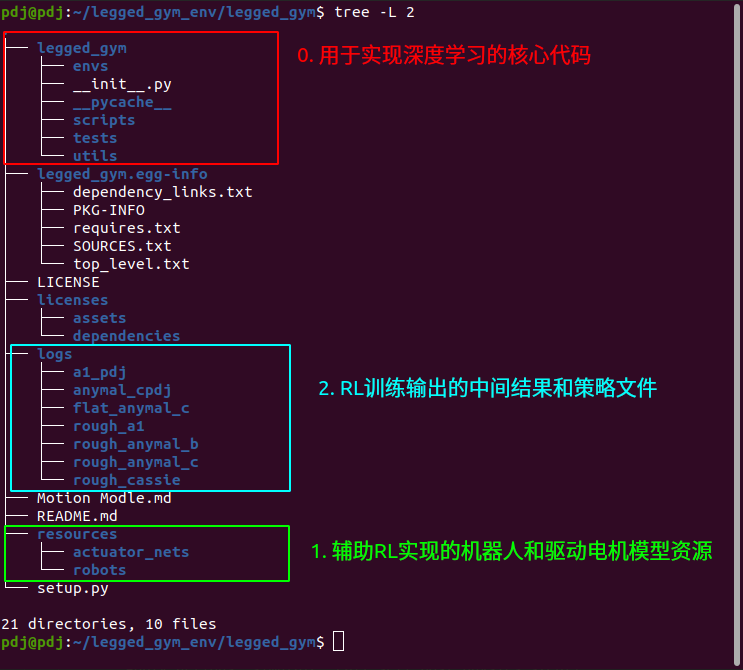
\includegraphics[width=0.8\linewidth]{legged_gym_overal_structure.png}
\end{figure}

整个例程库的文件结构如图\ref{fig:legged_gym_overal_structure}所示,图中标出了主要的三个文件:0. 用于实现深度学习的核心代码;1. 辅助实现RL的机器人电机模型和机器人物理模型; 2. RL训练输出的中间结果和最终的策略文件输出,其余的是一些基本的软件环境建立、开源协议等。这其中最重要的就是用于实现深度学习的核心代码部分(图\ref{fig:legged_gym_overal_structure}-0.),下面将介绍它的内容。

\subsection[\emph{legged\_gym}工具包]{\emph{legged\_gym}工具包}
legged\_gym文件是整个\emph{legged\_gym}工程中的核心部分,它的内部文件结构如图\ref{fig:legged_gym_structure}所示,主要包括三个部分:
\begin{enumerate}
  \item 训练的启动脚本;
  \item 辅助实现的脚本;
  \item 具体的模型实现文件;
\end{enumerate}

其中最值得关注的是第\emph{2. }部分关于具体环境模型实现的源码。它的文件路为:\emph{legged\_gym/legged\_gym/envs/*},内部的具体文件结构如图\ref{fig:legged_gym_envs_structure}所示,它包含了各种机器人模型的RL训练设置。我们重点关注机械狗类型的实现类(a1, anymal\_b, anymal\_c \ref{fig:legged_gym_envs_structure}-2.),它这些实现都是基于\emph{legged\_robot*.py}中定义的腿式机器人拓展类(\ref{fig:legged_gym_envs_structure}-1.)实现,而它的基类是(\ref{fig:legged_gym_envs_structure}-0.)类。

\begin{figure}
  \centering
  \subcaptionbox{\emph{legged\_gym} project structure\label{fig:legged_gym_structure}}
  {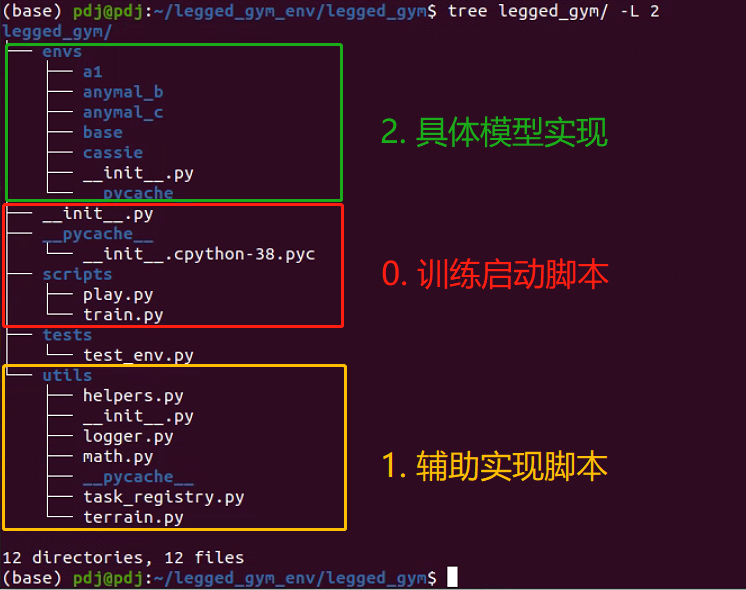
\includegraphics[width=0.44\linewidth]{legged_gym_structure.png}}
  \subcaptionbox{\emph{legged\_gym/envs} folder structure\label{fig:legged_gym_envs_structure}}
  {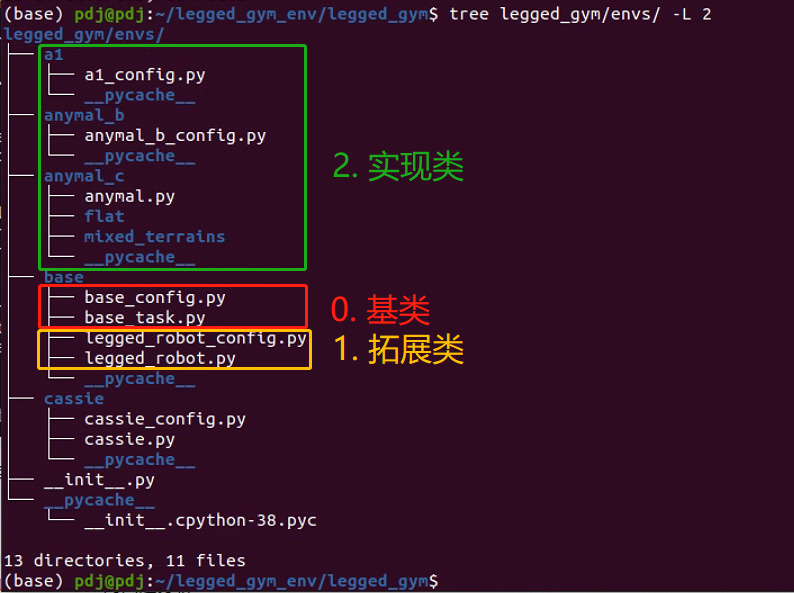
\includegraphics[width=0.47\linewidth]{legged_gym_envs_structure.png}}
\end{figure}

实际上整个RL训练还涉及到一个由ETH团队实现的用于深度学习的辅助库\href{https://github.com/leggedrobotics/rsl_rl}{\emph{rsl\_rl}},关于它的具体内容等待后续另做介绍。在接下来的内容中,我将会具体讲解关于腿式机器人的拓展类:\emph{LeggedRobot}类。以它为基础来对整个机器人的RL训练相关内容建立一个基本的认知。









\section[LeggedRobot类]{LeggedRobot类}
在\emph{legged\_gym}中用于足式机器人的仿真核心类就是\emph{LeggedRobot},它位于\emph{../legged\_gym/legged\_gym/envs/legged\_robot.py}文件中。\emph{LeggedRobot}的父类是\emph{BaseTask},它主要定义了整个RL训练过程的基本流程和一些待实现的方法模板,比较简单,这里不做过多介绍。实际上主要的方法实现位于\emph{LeggedRobot}中,下面将介绍它内部核心实现函数。


\subsection[从Isaac仿真环境中获取信息]{从Isaac仿真环境中获取信息}
\emph{legged\_gym}是在英伟达的Isaac仿真平台上实现训练的。关于Isaac平台的介绍在第\ref{section:isaac_gym}节中进行了介绍,它能够实现仿真和RL训练都在GPU平台上运行,拥有者很高效的学习效率。

\begin{figure}
  \centering
  \caption{\emph{function: \_init\_buffers} 这个函数处理了来自仿真环境中的数据;初始化了计算会用到的原始信息和将会生成的相关信息的内存空间;设置了关节点的位置偏移和PD增益。}
  \label{fig:legged_function_init_buffers}
  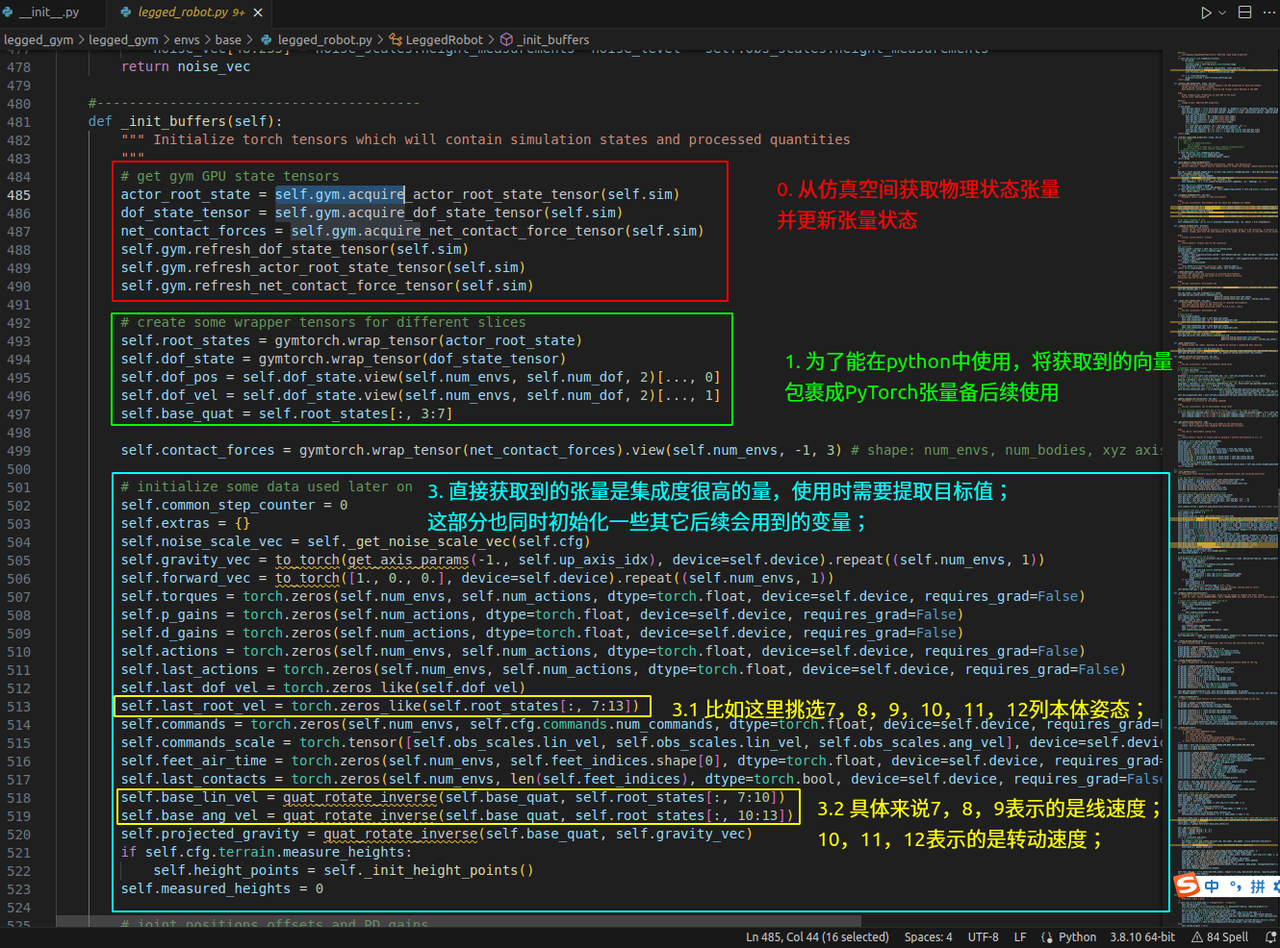
\includegraphics[width=1.0\linewidth]{legged_function_init_buffers.png}
\end{figure}

Isaac仿真平台提供Python接口来访问GPU中的数据,数据的交互是通过PyTorch张量实现的。如图\ref{fig:legged_function_init_buffers}所示,这是在\emph{内存初始化函数}中将isaac仿真平台中的实例的状态张量进行初始化(\ref{fig:legged_function_init_buffers}-0.),并通过包裹成PyTorch张量的形式进行使用(\ref{fig:legged_function_init_buffers}-1.)。由于Isaac仿真平台提供的张量是集成度很高的格式,再具体使用的时候还需要对数据进行有目的选择\ref{fig:legged_function_init_buffers}-2.)。这些数据的结构在节中也进行了简单的介绍,更具体的实现可以参考:\href{https://github.com/NVIDIA-Omniverse/IsaacGymEnvs}{IsaacGymEnvs}、\href{https://developer.nvidia.com/isaac-gym}{nvidia-isaac-gym}。



\subsection[LeggedRobot.step函数]{LeggedRobot.step函数}
在整个LeggedRobot类中\emph{step}函数是一个提纲挈领性的函数,它调用其余各个部分函数组件实现仿真的循环。外部函数对LeggedRobot类的激活就是通过调用其中的\emph{step}函数实现的。在\emph{legged\_gym}工程中\emph{step}函数的调用出现在这几个地方:\begin{enumerate}
  \item legged\_gym/legged\_gym/envs/base/base\_task.py中的\emph{BaseTask}类;
  \item legged\_gym/legged\_gym/scripts/play.py中的\emph{play}函数;
  \item legged\_gym/legged\_gym/scripts/test\_env.py中的\emph{test\_env}函数;
\end{enumerate}

\begin{figure}
  \centering
  \caption[LeggedRobot.step函数]{LeggedRobot.step函数}
  \label{fig:legged_function_step}
  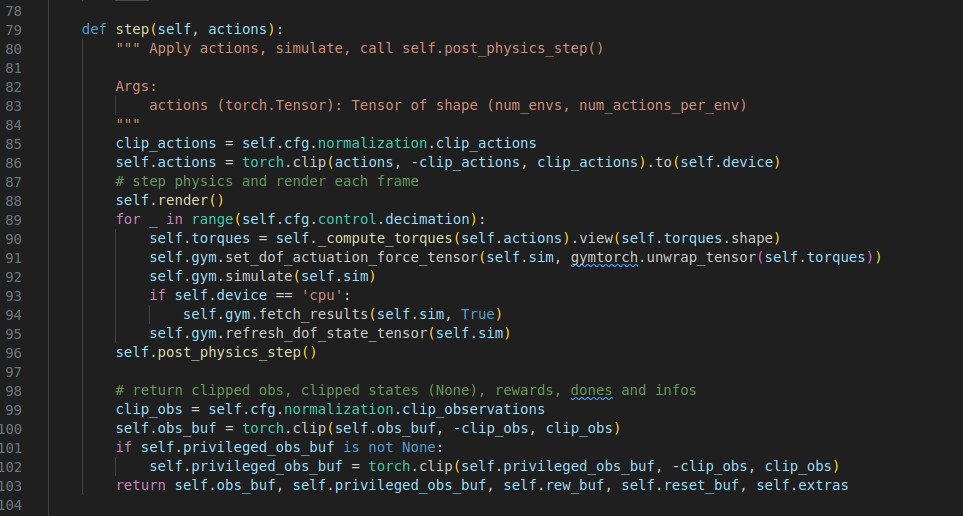
\includegraphics[width=1.0\linewidth]{legged_function_step.png}
\end{figure}

如图所示,\emph{step}函数的功能主要通过调用一下几个函数实现:\begin{enumerate}
  \item \emph{self.render}
  \item \emph{self.compute\_torques}
  \item \emph{self.gym.set\_dof\_actuation\_force\_tensor}
  \item \emph{self.gym.simulate}
  \item \emph{self.gym.fetch\_results}
  \item \emph{self.gym.refresh\_dof\_state\_tensor}
  \item \emph{self.post\_physics\_step}
\end{enumerate}

这其中比较关于仿真环境的\emph{self.gym.xxx}我们暂时不讨论,下面主要关注这三个:\emph{self.render};\emph{self.compute\_torques};\emph{self.post\_physics\_step}。



\subsection[self.render函数]{self.render函数}
如图\ref{fig:legged_function_render}所示,\emph{self.render}函数在\emph{LeggedRobot}的父类\emph{BaseTask}中定义和实现,主要的作用就是处理CPU端监测、界面和键盘交互的一些操作,比如关闭窗口等。
\begin{figure}
  \centering
  \caption[LeggedRobot.render函数]{LeggedRobot.render函数}
  \label{fig:legged_function_render}
  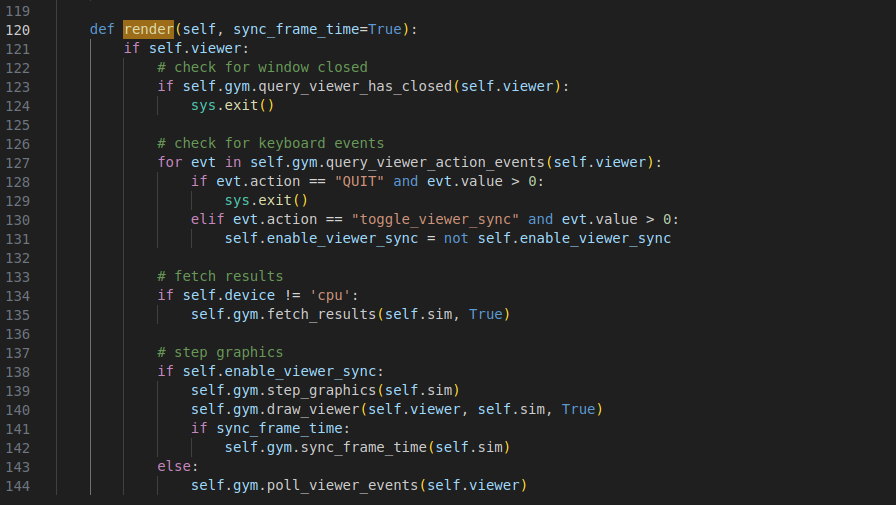
\includegraphics[width=1.0\linewidth]{legged_function_render.png}
\end{figure}

\subsection[self.compute\_torques函数]{self.compute\_torques函数}
如图\ref{fig:legged_function_compute_torques}所示,\emph{self.\_compute\_torques}函数的作用是根据输入的控制动作计算机器人各个关节点的扭矩,目标的的控制可能是基于位置的、基于速度的或者直接基于缩放后的扭矩的。采用的控制方法是PD控制。计算后的扭矩结果会被发送到仿真环境中。
\begin{figure}
  \centering
  \caption[LeggedRobot.\_compute\_torques函数]{LeggedRobot.\_compute\_torques函数}
  \label{fig:legged_function_compute_torques}
  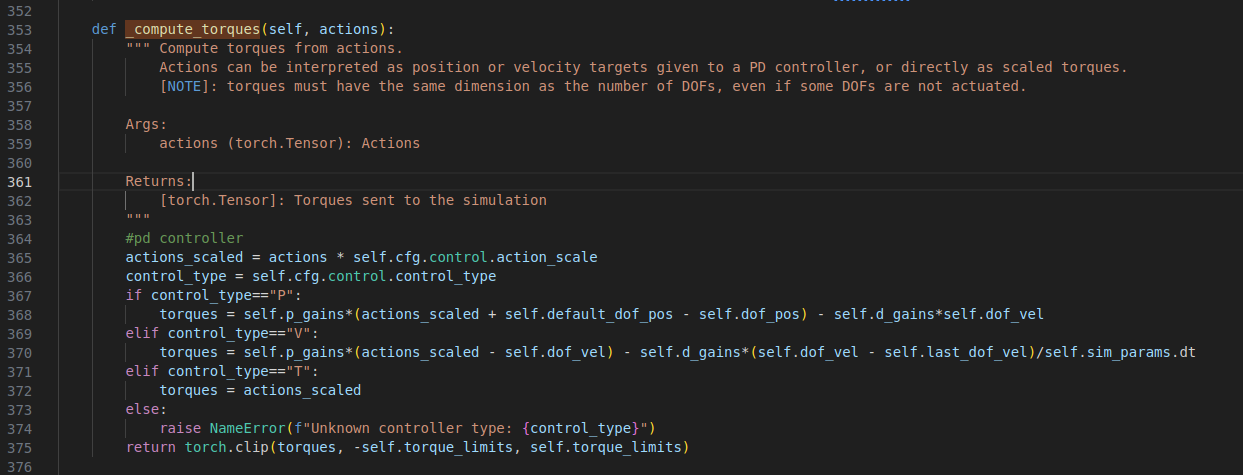
\includegraphics[width=1.0\linewidth]{legged_function_compute_torques.png}
\end{figure}

\subsection[self.post\_physics\_step函数]{self.post\_physics\_step函数}
如图\ref{fig:legged_function_post_physics_step}所示,\emph{self.post\_physics\_step}函数的主要作用包括监测终止条件、计算观测和奖励等。相关的函数包括:\begin{enumerate}
  \item \emph{self.\_post\_physics\_step\_callback}
  \item \emph{self.check\_termination}
  \item \emph{self.compute\_reward}
  \item \emph{self.reset\_idx}
  \item \emph{self.compute\_observations}
  \item \emph{self.\_draw\_debug\_vis}
\end{enumerate}
\begin{figure}
  \centering
  \caption[LeggedRobot.post\_physics\_step函数]{LeggedRobot.post\_physics\_step函数}
  \label{fig:legged_function_post_physics_step}
  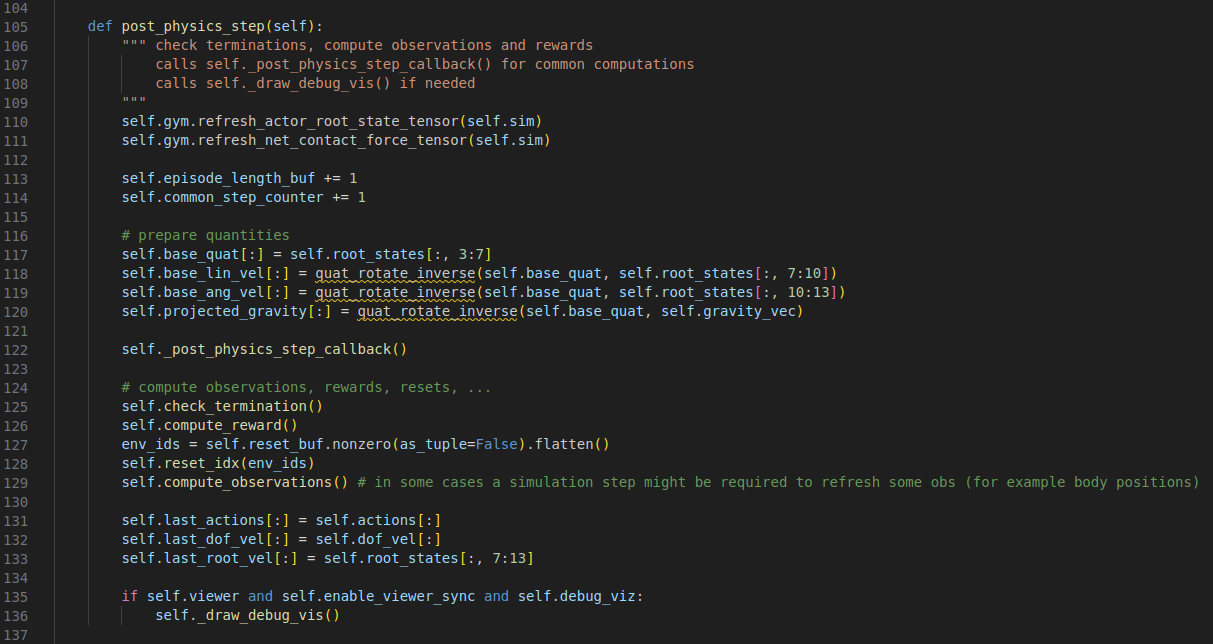
\includegraphics[width=1.0\linewidth]{legged_function_post_physics_step.png}
\end{figure}

这些被调用的函数中最值得关注的是第(3)条:\emph{self.compute\_reward}和\emph{self.compute\_observations}。\emph{self.compute\_reward}就是RL问题中的奖励计算函数,包含着十几条具体的奖励计算定义。\emph{self.compute\_observations}就是RL问题中的观测状态计算函数。这两个函数的具体定义将在接下来的两节中介绍。



\subsection[self.compute\_observations函数]{self.compute\_observations函数}
如图\ref{fig:legged_function_compute_observations}所示,\emph{self.compute\_observations}函数的作用包括计算本体感知、添加外部感知、添加为感知噪声。
\begin{figure}
  \centering
  \caption[LeggedRobot.compute\_observations函数]{LeggedRobot.compute\_observations函数}
  \label{fig:legged_function_compute_observations}
  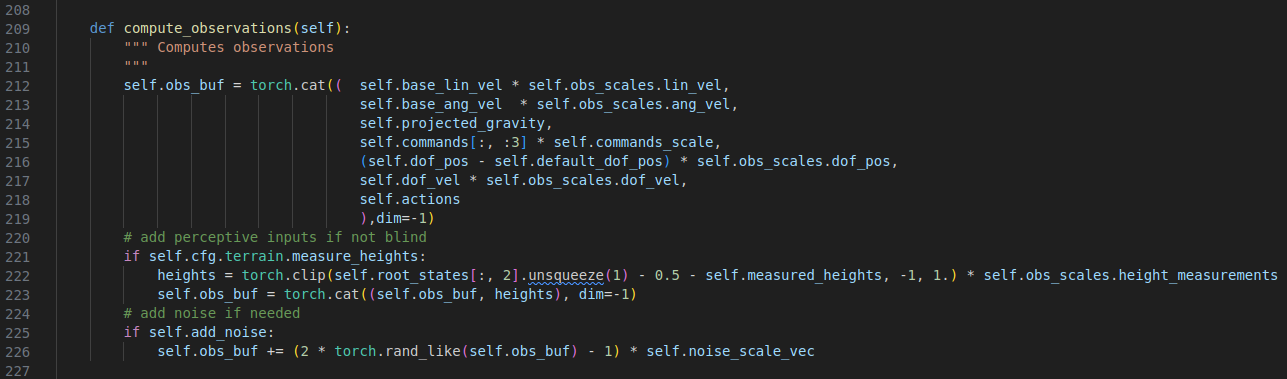
\includegraphics[width=1.0\linewidth]{legged_function_compute_observations.png}
\end{figure}

\subsection[self.compute\_reward函数]{self.compute\_reward函数}
如图\ref{fig:legged_function_compute_reward}所示,\emph{self.compute\_reward}函数会从一系列的奖励函数中计算总和。这一系列的奖励函数都定义都预先用\emph{self.\_prepare\_reward\_function}进行了打包,因此在\emph{self.compute\_reward}函数中只需要遍历访问和累加即可。这些函数的具体计算定义也在\emph{LeggedRobot}类中,由于数量过多就不一一展示了,大致如图\ref{fig:legged_function_all_rewards}所示。
\begin{figure}
  \centering
  \caption[LeggedRobot.compute\_reward函数]{LeggedRobot.compute\_reward函数}
  \label{fig:legged_function_compute_reward}
  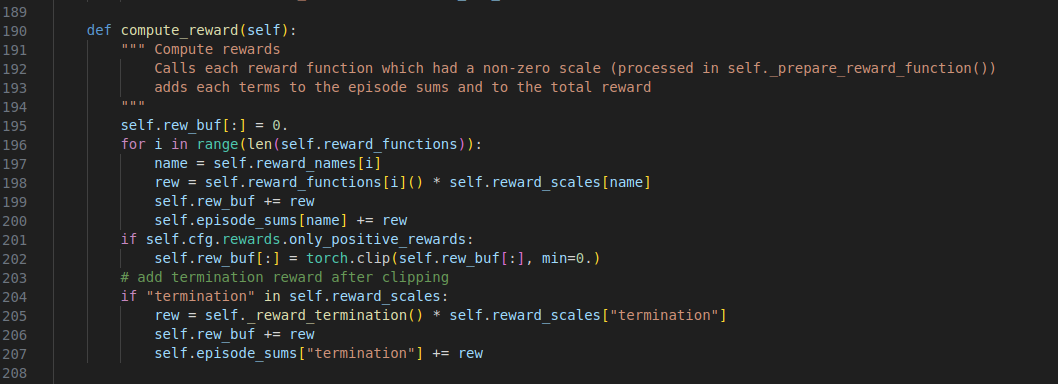
\includegraphics[width=1.0\linewidth]{legged_function_compute_reward.png}
\end{figure}

\begin{figure}
  \centering
  \caption[LeggedRobot.xxx奖励函数]{LeggedRobot.xxx奖励函数}
  \label{fig:legged_function_all_rewards}
  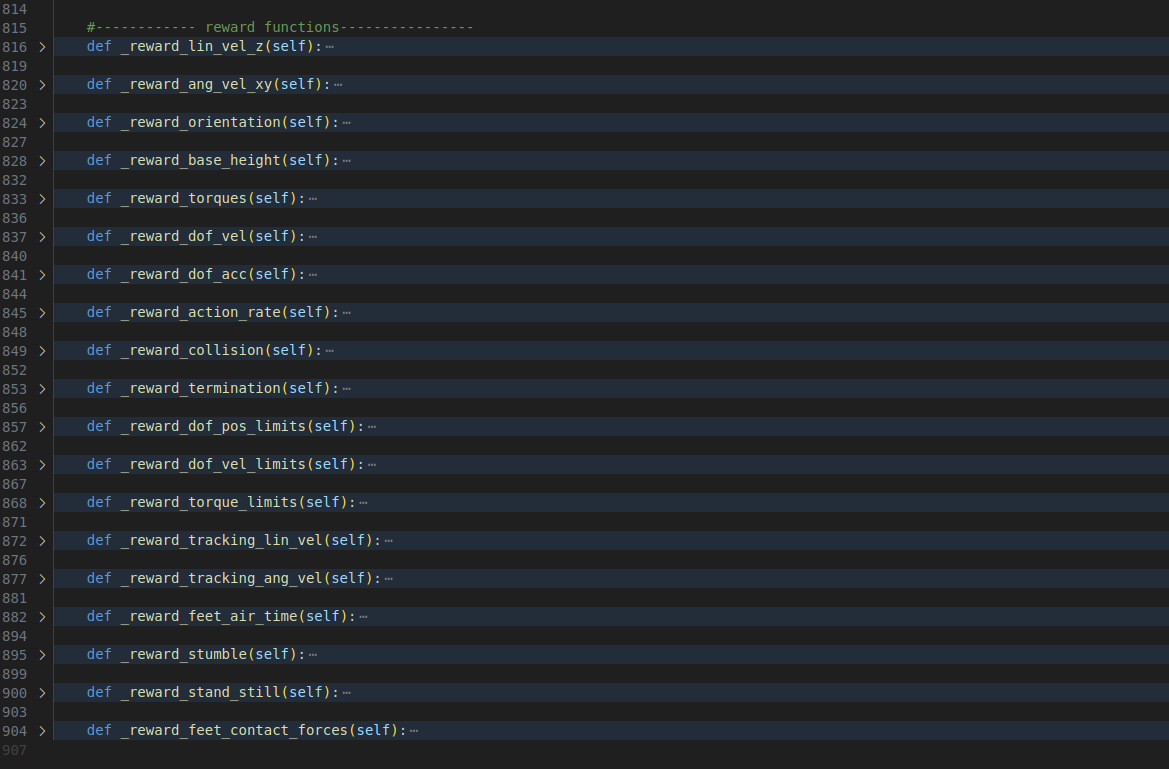
\includegraphics[width=1.0\linewidth]{legged_function_all_rewards.png}
\end{figure}

这些奖励的计算过程会考虑到他们的系数,可以根据不同机器人的情况方便地调节各个奖励的贡献。这些系数初始定义在\emph{LeggedRobot}类相应的配置类\emph{LeggedRobotCfg}类里面,如图\ref{fig:legged_cfg_rewards}所示。

\begin{figure}
  \centering
  \caption[LeggedRobotCfg.rewards函数]{LeggedRobotCfg.rewards函数}
  \label{fig:legged_cfg_rewards}
  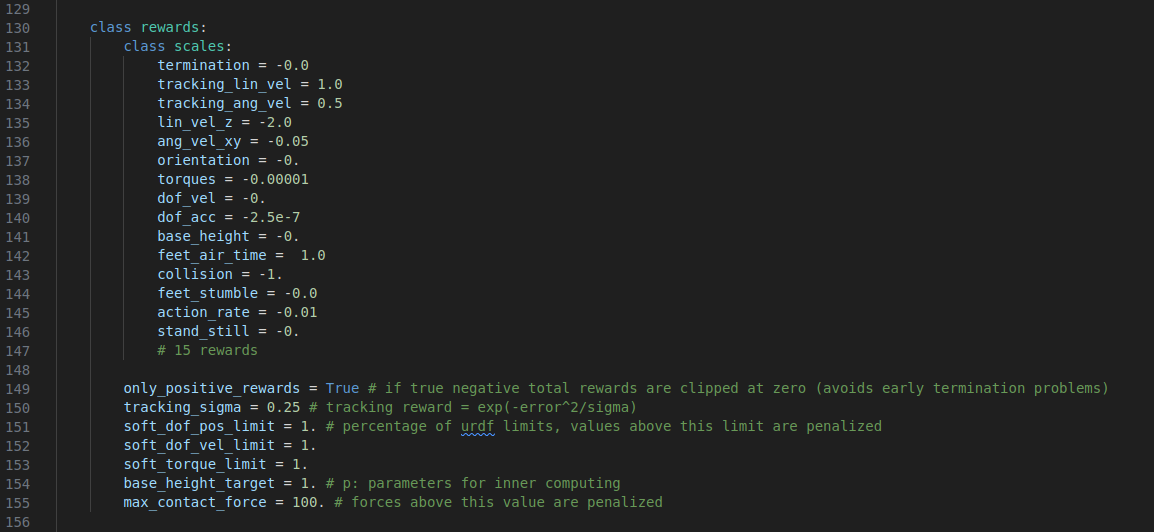
\includegraphics[width=1.0\linewidth]{legged_cfg_rewards.png}
\end{figure}



